%DEFINES THE PREAMBLE FOR STANDARD SMARTASS ASSIGNMENT

\documentclass[10pt,fleqn]{article}

%\usepackage{epsf}
\usepackage{amsmath}
\usepackage{amssymb} 
\usepackage{cancel} %cancelled numbers 
%\usepackage{lcg} %random numbers generator
\usepackage{ifthen} %logical constructs
<<<<<<< HEAD
=======
\usepackage{enumerate}
\usepackage{siunitx}

>>>>>>> Added additional default LaTeX packages.

\newif\ifpdf
\ifx\pdfoutput\undefined
\pdffalse
\else
\pdfoutput=1
\pdftrue
\fi

\ifpdf
\usepackage[pdftex]{overpic}
\usepackage[pdftex]{graphicx}
\pdfcompresslevel=9
\pdfpagewidth=215truemm 
\pdfpageheight=297truemm
\pdfhorigin=1truein
\pdfvorigin=1truein
\else
\usepackage{overpic}
\usepackage{graphicx}
\fi

\setlength{\textwidth}{185.0mm}
\setlength{\textheight}{660pt}
\setlength{\oddsidemargin}{-15.0mm}
\setlength{\evensidemargin}{-15.0mm}
\setlength{\headsep}{0pt}
%\setlength{\topmargin}{-29.0truemm}
\setlength{\parindent}{0.0truemm}

\renewcommand {\theenumi}{\bf \arabic{enumi}}
\renewcommand {\theenumii} {\textbf{\arabic {enumii}}}
\renewcommand {\theenumiii} {\textbf {\roman{enumiii}}}


\begin{document}
%%BEGIN DEF 
%definition of variables/modules used
%There needs to be a graphic file GraphsForFunctionGraphsCompositeTemplate.eps included somewhere 
%INSERT THIS WHERE YOU WANT A PICTURE:
%\begin{figure}[tbh]
%\centerline{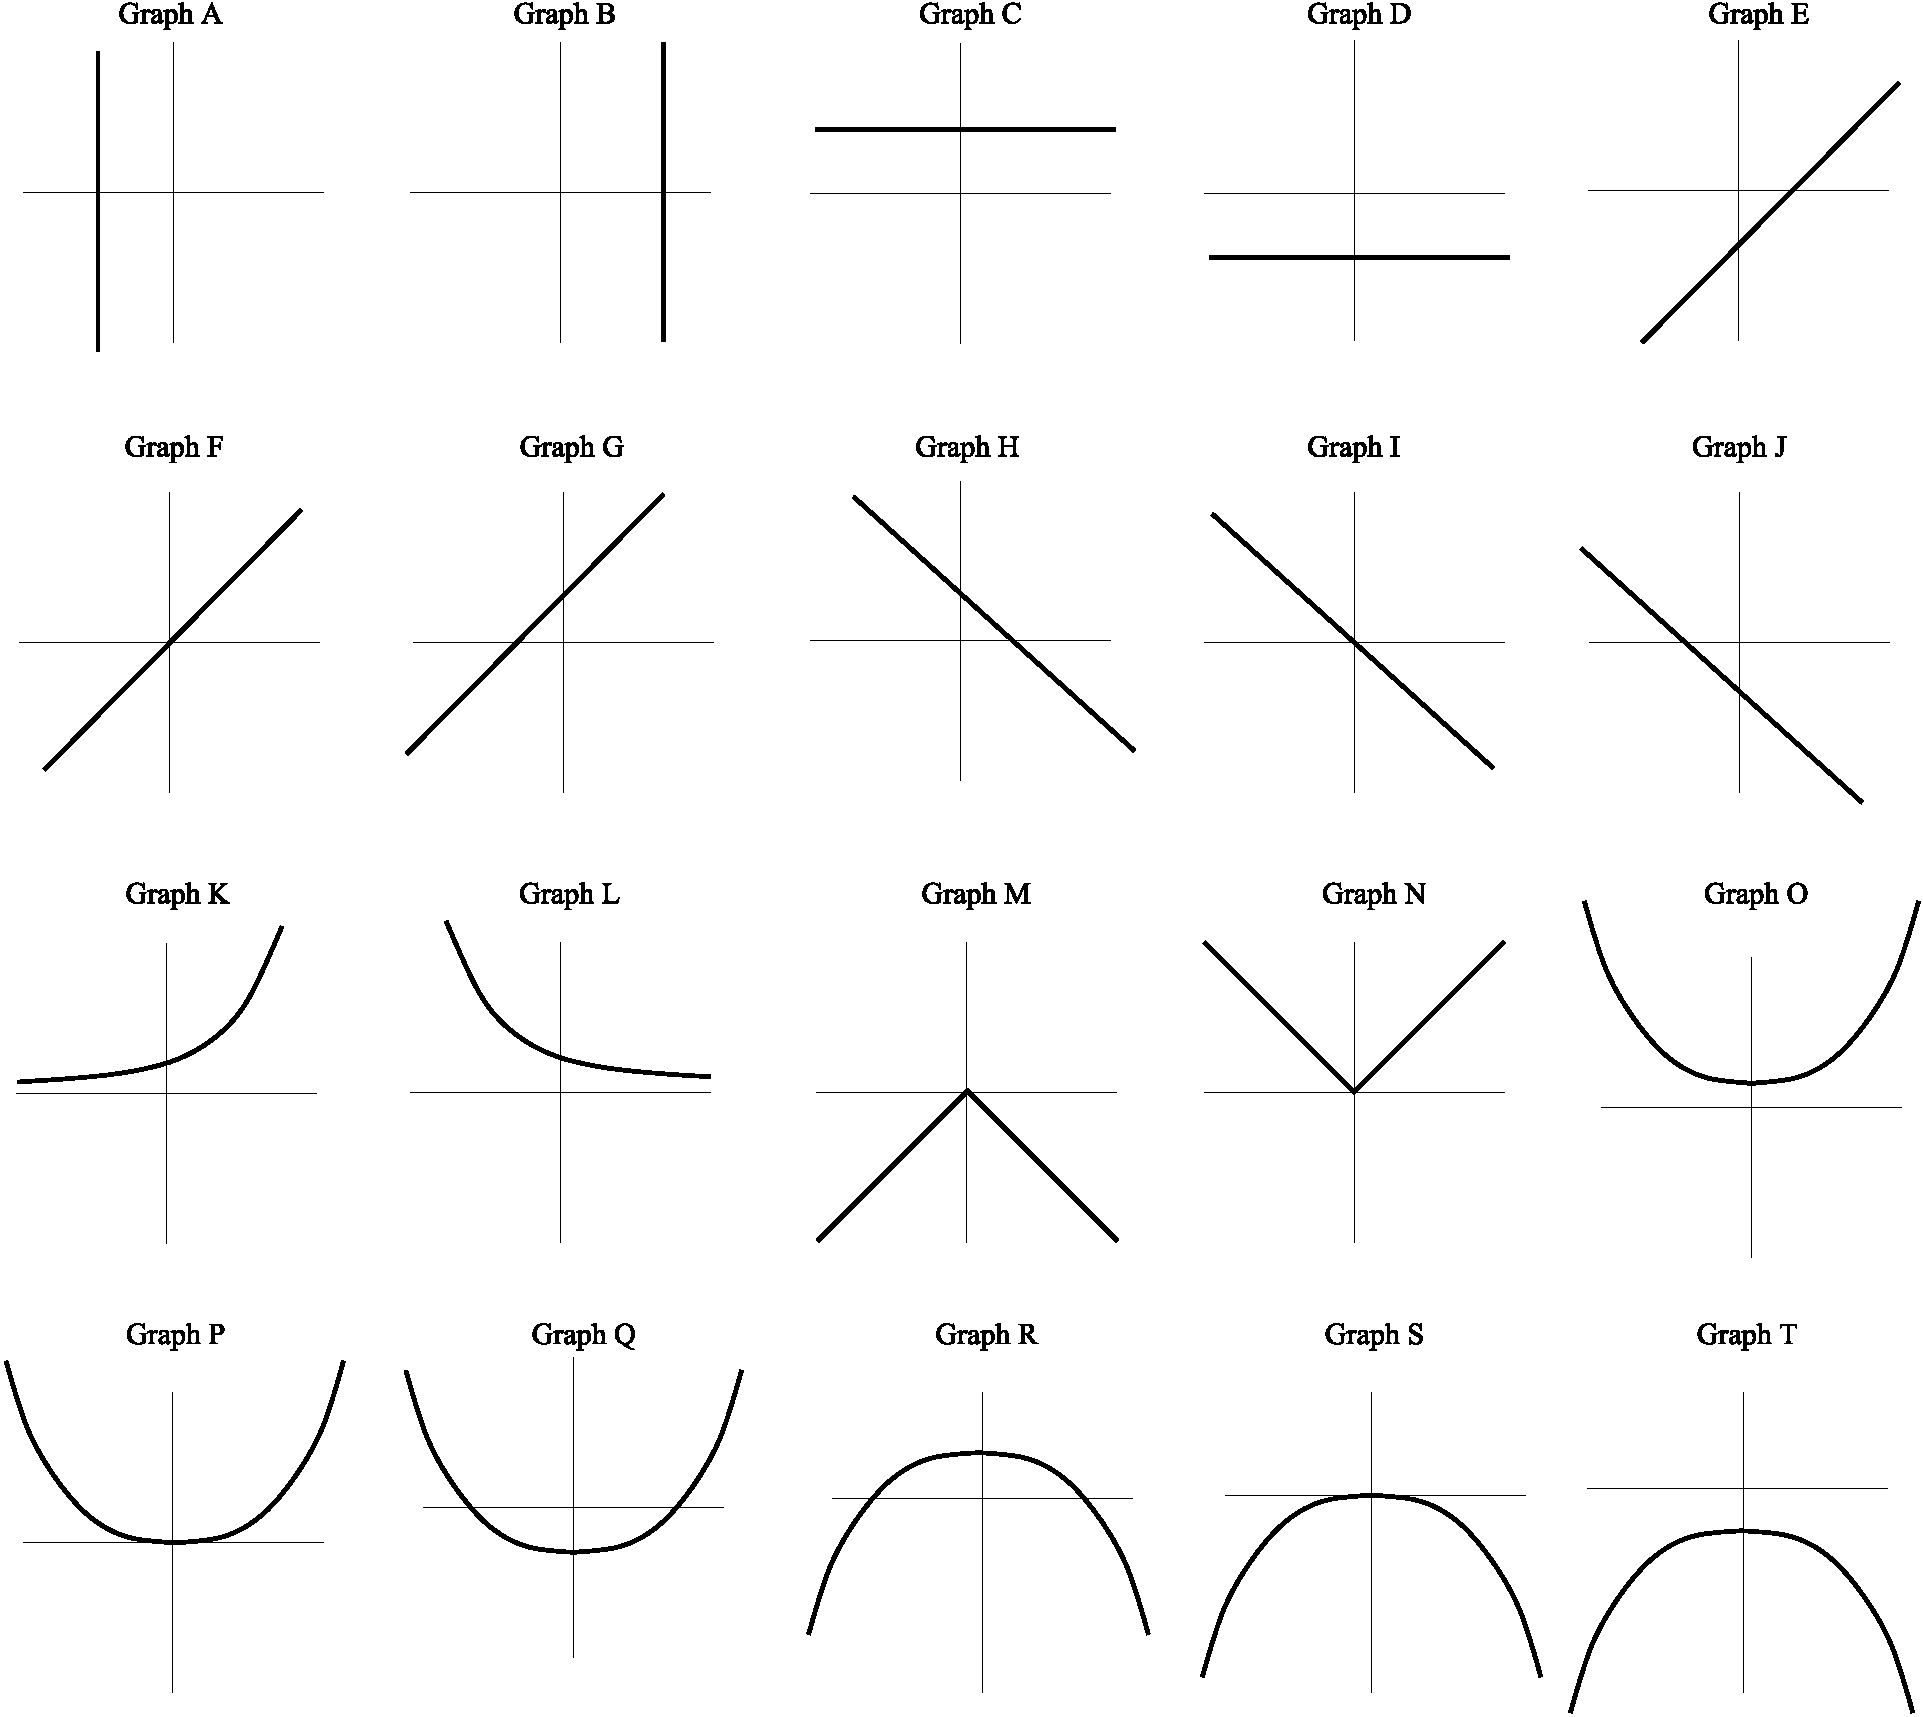
\includegraphics[height=150mm]{GraphsForFunctionGraphsCompositeTemplate.pdf}}
% \caption{Graphs of various equations.}\label{Fi:GraphsForFunctionGraphsCompositeTemplate}
%\end{figure}

#<
FunctionGraphsCompositeModule v1;
#>

%%END DEF

%%BEGIN QUESTION

\begin{figure}[tbh]
\centerline{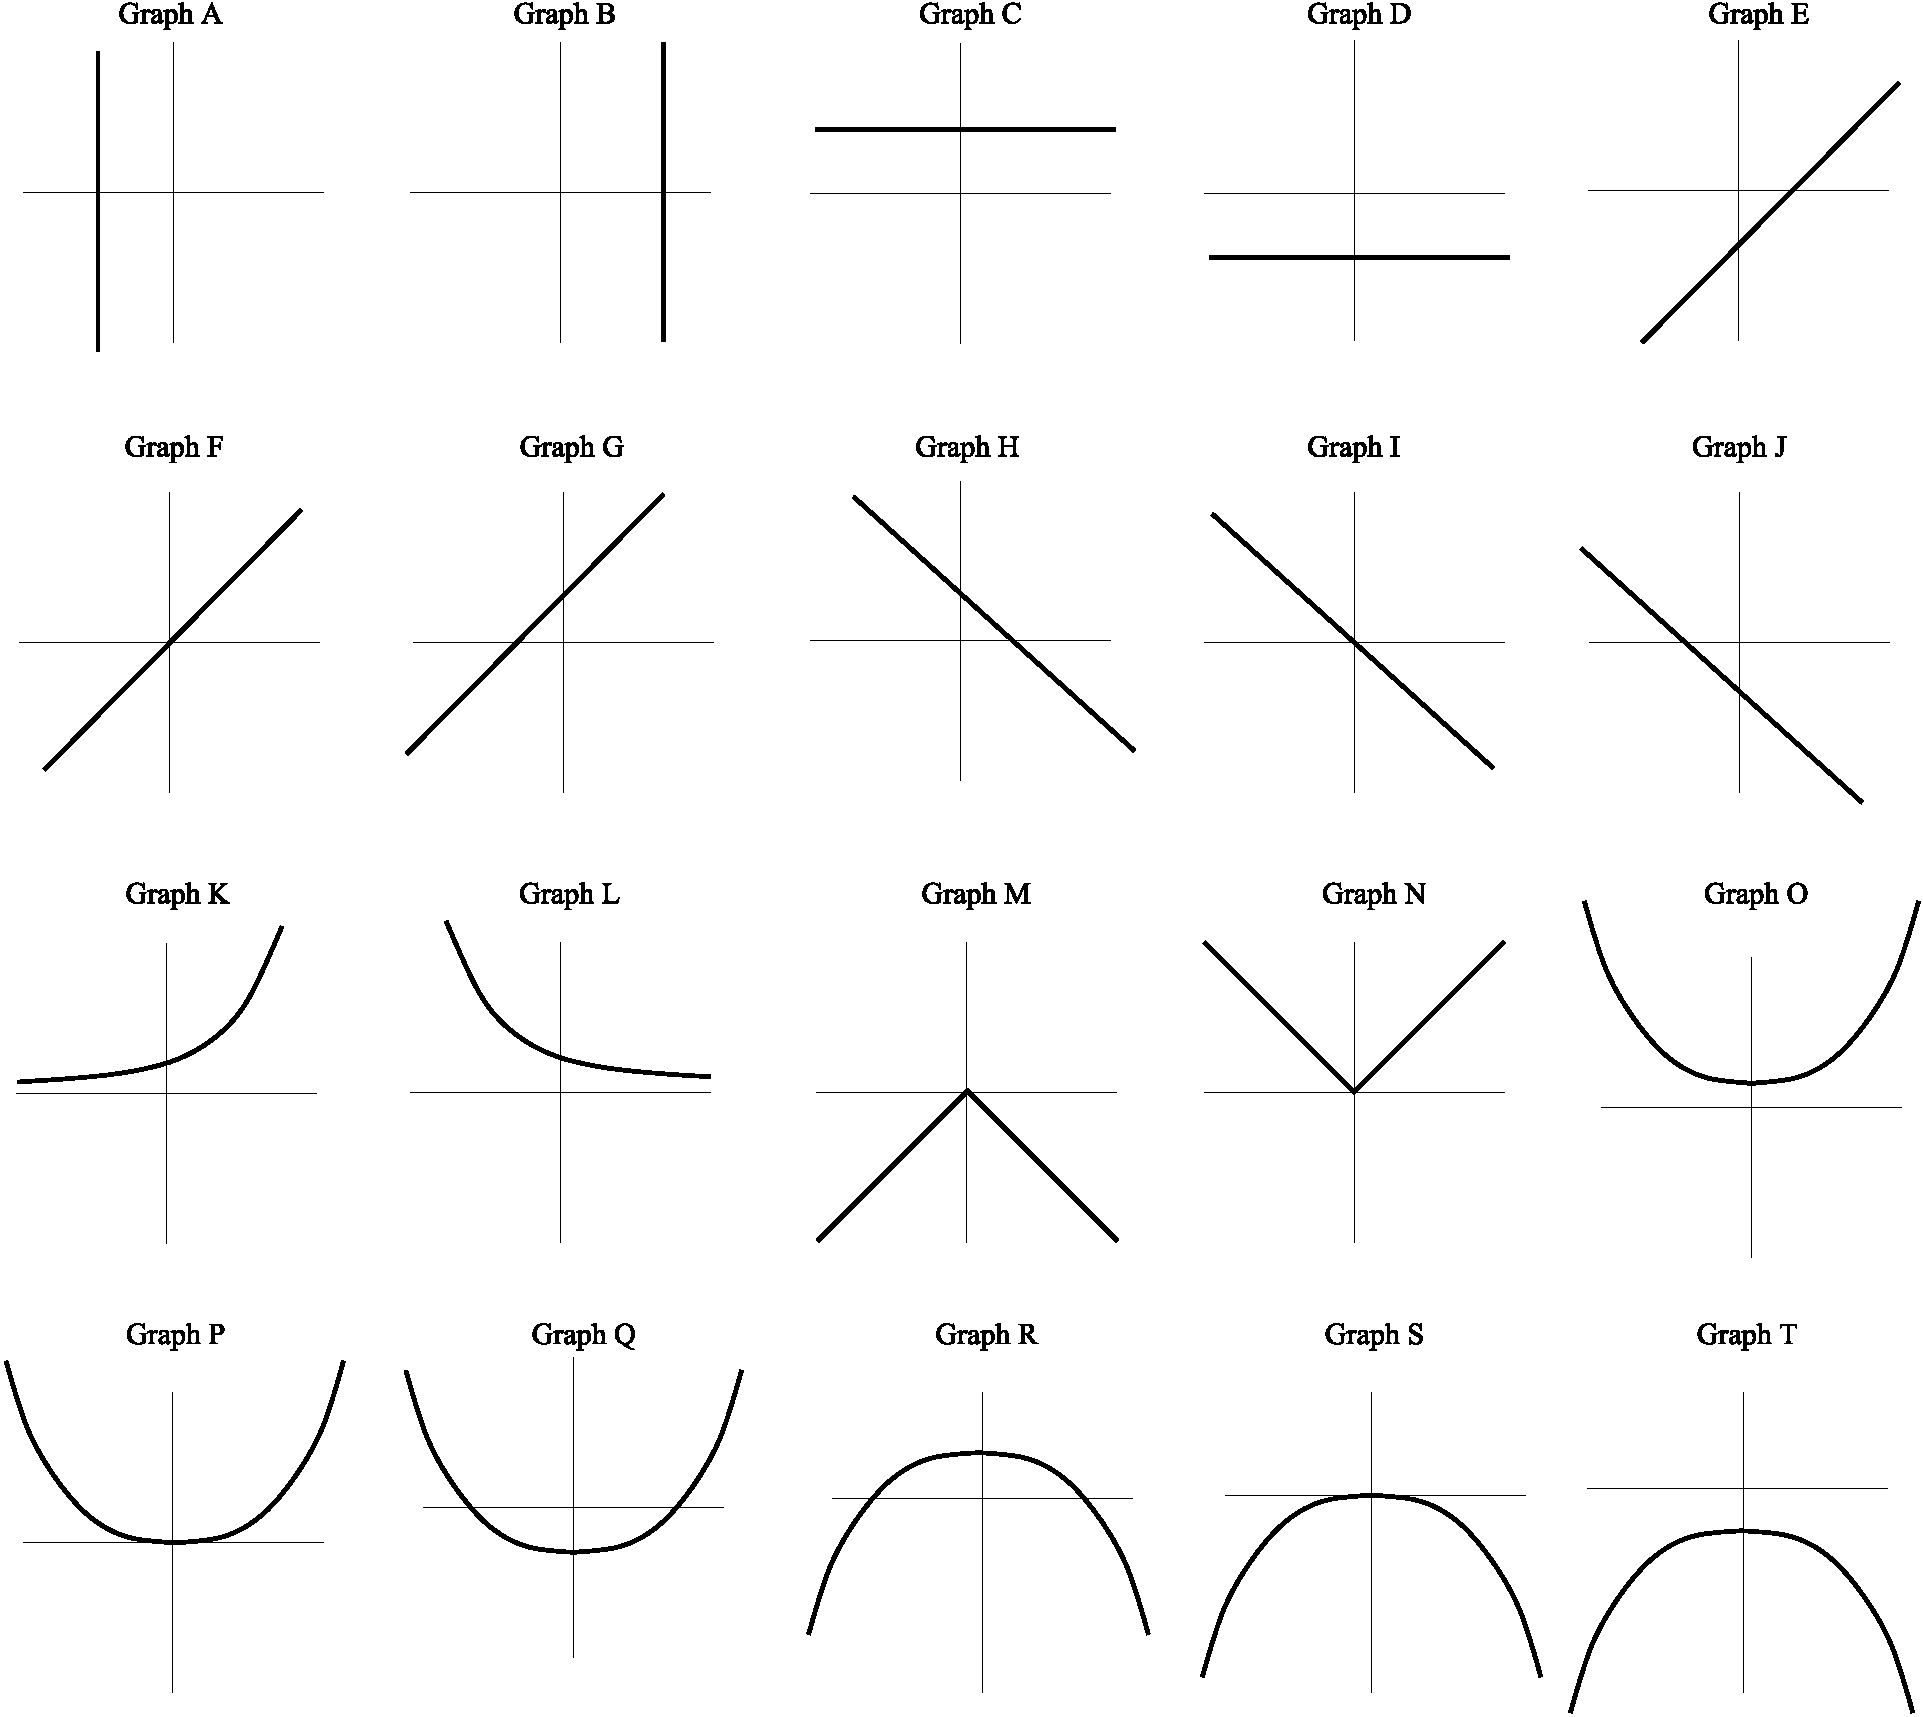
\includegraphics[height=150mm]{GraphsForFunctionGraphsCompositeTemplate.pdf}}
 \caption{Graphs of various equations.}\label{Fi:GraphsForFunctionGraphsCompositeTemplate}
\end{figure}

There are eight equations given in this question and you need to match each equation with its corresponding graph. The 
graphs are shown in Figure~\ref{Fi:GraphsForFunctionGraphsCompositeTemplate}.
\begin{enumerate}
\item
#<v1.question1#> 
\item
#<v1.question2#> 
\item
#<v1.question3#> 
\item
#<v1.question4#> 
\item
#<v1.question5#>
\item
#<v1.question6#>
\item
#<v1.question7#>
\item
#<v1.question8#>

\end{enumerate}

%%END QUESTION

%%BEGIN SOLUTION
\begin{enumerate}
\item
#<v1.solution1#>.\\
\item
#<v1.solution2#>.\\
\item
#<v1.solution3#>.\\
\item
#<v1.solution4#>.\\
\item
#<v1.solution5#>.\\
\item
#<v1.solution6#>.\\
\item
#<v1.solution7#>.\\
\item
#<v1.solution8#>. \\

\end{enumerate}
%%END SOLUTION

%%BEGIN SHORTANSWER
\begin{enumerate}
\item
#<v1.shortanswer1#>
\item
#<v1.shortanswer2#>
\item
#<v1.shortanswer3#>
\item
#<v1.shortanswer4#>
\item
#<v1.shortanswer5#>
\item
#<v1.shortanswer6#>
\item
#<v1.shortanswer7#>
\item
#<v1.shortanswer8#> 

\end{enumerate}

%%END SHORTANSWER

\end{document}
